\documentclass[a4paper,12pt]{article}
\usepackage[utf8]{inputenc}      % Codificación UTF-8 para caracteres en español
\usepackage[T1]{fontenc}         % Buena salida de fuentes
\usepackage[spanish]{babel}      % Traducción de elementos automáticos al español
\usepackage{lmodern}             % Fuente mejorada
\usepackage[hidelinks]{hyperref} % Para enlaces, [hidelinks] elimina el reborde azul del .pdf
\usepackage{graphicx}            % Para incluir imágenes (PNG)
\usepackage{float}               % Para anclar las imagenes a una posicion fija
%\usepackage{graphics-external}   Tambien da error
\usepackage{bytefield}           % Para dibujar diagramas PDU
\usepackage{geometry}            % Para ajustar márgenes
\geometry{left=2.5cm, right=2.5cm, top=3cm, bottom=3cm}

\title{El protocolo IPv6}
\author{Martín Moloeznik, Nicolás Paz Reyes\\[0.5em]
Repositorio: \url{https://github.com/tu_usuario/tu_repositorio}}
\date{\today}

\begin{document}

% Carátula
\begin{titlepage}
  \centering
  \vspace*{2cm}
  {\large \textbf{El protocolo IPv6}}\\[1.5cm]
  
  {\large Integrantes:}\\
   \bigskip
  {\large Martín Moloeznik, Nicolás Paz Reyes} \\[0.5cm]
  {\large {martinmoloeznik@gmail.com}, {rubenpaz2105@gmail.com}} \\[0.5cm]
  \bigskip
  {\large Repositorio: \url{https://github.com/N1C0-P4Z/Protocolo-IPv6}}\\[1cm]
  
  \vfill
  {\large \today}
\end{titlepage}

% Índice (opcional)
\tableofcontents
\newpage

% Sección de Introducción
\section{Introducción}
El protocolo IPv6 fue desarrollado para reemplazar a IPv4 debido a la necesidad de una mayor cantidad de direcciones IP en el mundo. Dentro de IPv6 existen mecanismos esenciales para la configuración de direcciones y la comunicación entre dispositivos, entre los cuales se destacan SLAAC, EUI-64 y el protocolo Neighbor Discovery (NDP).

% Sección 1: Escenarios y Configuraciones
\section{IPv6 SLAAC and EUI-64 Basics}
\subsection{Configuración del Router en IPv6}
\begin{figure}[H]
  \centering
  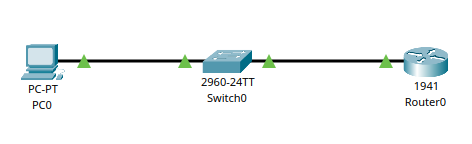
\includegraphics[width=0.7\textwidth]{imagenes/lab1.png}
  \caption{Red a ensayar}
  \label{fig:lab1}
\end{figure}

Aquí se detalla la configuración necesaria en el router, incluyendo la activación de IPv6, asignación de direcciones LLA y GUA, y otros comandos.

\subsection{Explicacion algoritmo EUI-64}
   La pc se autoconfigura su Link Local Addres siguiendo los pasos a continuacion:
\bigskip
+
\begin{bytefield}[boxformatting={\centering\itshape},bitwidth = 1.1em]{32}
  \begin{rightwordgroup}{Algoritmo \\ EUI-64}

    \bitbox{16}{48 bit MAC} & \bitbox{16}{00-E0-F9-98-8A-07}\\
    \bitbox{16}{Separa al medio} & \bitbox{16}{00-E0-F9 \hspace{0.45cm} | \hspace{0.45cm} 98-8A-07}\\
    \bitbox{16}{Insertar FF-FE} & \bitbox{16}{00-E0-F9 \textbf{FF-FE} 98-8A-07}\\
    \bitbox{16}{Primeros dos hexa a binario} & \bitbox{16}{0000-0000-E0-F9  \textbf{FF-FE} 98-8A-07}\\
    \bitbox{16}{Se invierte el septimo bit} & \bitbox{16}{0000-00\textbf{1}0-E0-F9  \textbf{FF-FE} 98-8A-07}\\
    \bitbox{16}{64 bits host interface ID} & \bitbox{16}{\textbf{02}-E0-F9-\textbf{FF-FE}-98-8A-07}\\
    \bitbox{16}{Link Local Address} & \bitbox{16}{FE80::\textbf{2E0:F9FF:FE98:8A07}}
  \end{rightwordgroup}
\end{bytefield}

\bigskip
\begin{bytefield}[boxformatting={\centering\itshape},bitwidth = 1.1em]{32}
  \bitheader{0,4,12,32} \\
  \bitbox{4}{Ver:6} & \bitbox{8}{TRFC} & \bitbox{20}{FLOW LABEL}\\
  \bitbox{16}{PL:12} & \bitbox{8}{NEXT:0x3a} & \bitbox{8}{HOP LIMIT:255}\\ 
  \begin{rightwordgroup}{Link Local\\ Address}
    \wordbox{2}{SRC IP:FE80::2E0:F9FF:FE98:8A07}
  \end{rightwordgroup}\\
  \begin{rightwordgroup}{All Routers\\ Multicast \\address}
    \wordbox{2}{DEST IP:FF02::2}
  \end{rightwordgroup}
\end{bytefield}

% Sección 2: Escenario 2: Neighbor Discovery
\section{Escenario 2: Neighbor Discovery y NDP}
En esta sección se describe el proceso de descubrimiento de vecinos en IPv6, incluyendo:
\begin{itemize}
  \item Configuración de las interfaces en el router y dispositivos.
  \item Flujo de mensajes de NDP y explicación de cada uno (por ejemplo, RS y RA).
  \item Análisis de los PDUs involucrados y la conversión de direcciones MAC.
\end{itemize}

% Sección de Conclusiones
\section{Conclusiones}
Aquí se sintetizan los resultados obtenidos y se discuten las ventajas y desventajas de la autoconfiguración en IPv6, así como el impacto del proceso de Neighbor Discovery en el rendimiento de la red.

% Sección de Referencias
\section{Referencias}
Para la elaboracion de este informe utilizamos el contenido de los siguientes videos. 
\begin{itemize}
  \item \textbf{Video 1:} “IPv6 SLAAC and EUI-64 Basics in Packet Tracer”, Dan Alberghetti, 2019, at \url{https:
  //www.youtube.com/watch?v=yMK1NVHksDE}.
  \item \textbf{Video 2:} “IPv6 NDP and ICMPv6 using Packet Tracer”, Dan Alberghetti, 2020, at \url{https://www.
  youtube.com/watch?v=y2GpG9aOIFI}
  \item \textbf{Video 3:} “Detección de vecinos IPv6 (Packet Tracer Lab 9.3.4)”, RedesNetw channel, 2022, at \url{https://www.youtube.com/watch?v=ZBVXbgF39gw}
+\end{itemize}

\end{document}
